% ============ Section IV: Validation and Methodology (Member 1) ============
% Topic 9 asks for "Validation: time-based split by month" as Section 4; the brief's general
% section list asks for the methodology content (pipeline, models, tuning, metrics, versions).
% Both are covered here.
\section{Validation and Methodology}
\label{sec:method}

Fig.~\ref{fig:pipeline} gives an overview of the whole pipeline. One rule is behind every choice in
this section: no information from a later month, and nothing from the test months, may reach a model
or a decision before that model is evaluated.

\begin{figure*}[!t]
\centering
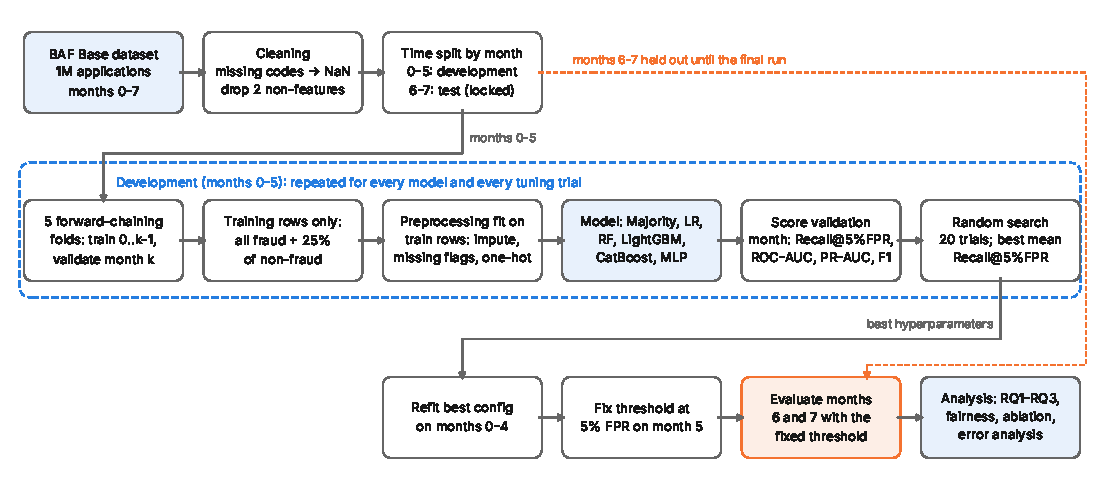
\includegraphics[width=\textwidth]{figures/pipeline.pdf}
\caption{Experimental pipeline. Months 0--5 are used for model selection with five forward-chaining
folds, and all sampling and preprocessing is fitted on the training rows of each fold only. The best
configuration of each model is refitted on months 0--4, its decision threshold is fixed at a 5\%
false positive rate on month 5, and it is then evaluated once on months 6 and 7.}
\label{fig:pipeline}
\end{figure*}

\subsection{Time-Based Split by Month}
\label{sec:method-split}

We follow the split of the original BAF paper \cite{jesus2022turning}. Months 0--5 are used for
development, and months 6 and 7 are kept as the test period. The months are never shuffled. Inside
the development period we use forward-chaining (expanding window) cross-validation
\cite{cerqueira2020evaluating}. Fold $k$ ($k=1,\dots,5$) trains on months $0$ to $k-1$ and validates
on month $k$, so each validation month comes strictly after the data the model was trained on.
Table~\ref{tab:folds} gives the size and fraud rate of each fold. With five folds we can report the
mean and standard deviation of every metric and still respect the order of time, which a shuffled
$k$-fold split would not do \cite{kaufman2012leakage}. The downside is that early folds train on less
data than later ones, so the variation between folds comes from both training size and drift. We
keep this in mind when we read the standard deviations.

\begin{table}[!t]
\centering
\caption{Forward-chaining folds on the development months (training sizes before sampling).}
\label{tab:folds}
\footnotesize
\setlength{\tabcolsep}{3.5pt}
\begin{tabular}{ccrrrr}
\hline
Fold & Train mon. & Train rows & Fraud & Val. mon. & Fraud \\
\hline
1 & 0 & 132,440 & 1.13\% & 1 & 0.94\% \\
2 & 0--1 & 260,060 & 1.04\% & 2 & 0.87\% \\
3 & 0--2 & 397,039 & 0.98\% & 3 & 0.92\% \\
4 & 0--3 & 547,975 & 0.97\% & 4 & 1.14\% \\
5 & 0--4 & 675,666 & 1.00\% & 5 & 1.18\% \\
\hline
\end{tabular}
\end{table}


After model selection, each model is refitted with its best hyperparameters on months 0--4. Month 5
is only used to fix the decision threshold (and, for the boosting models and the MLP, for early
stopping), and then months 6 and 7 are scored once. We chose this instead of refitting on all of
months 0--5, because setting the threshold on the test months would mean tuning on test data. The
original BAF study set its threshold on the test period and mentioned a separate validation split as
future work \cite{jesus2022turning}. Since our threshold comes from an earlier month, the false
positive rate on months 6 and 7 will not be exactly 5\%. We report the value that is actually
reached, because the gap is itself a sign of drift (RQ2).

\subsection{Preprocessing}
\label{sec:method-prep}

The cleaning steps in Section~\ref{sec:dataset} (decoding the missing values and removing
\texttt{month} and \texttt{device\_fraud\_count}) do not learn anything from the data, so they are
applied to the whole file once. Every step that does learn from the data is part of a scikit-learn
pipeline \cite{pedregosa2011scikit} and is fitted inside each fold on the training rows only:
{\sloppy
\begin{itemize}
  \item numeric features: missing values are replaced by the training median, and a 0/1 indicator
        column is added for each feature that had missing values, since missingness itself is
        related to fraud (Section~\ref{sec:dataset});
  \item categorical features (\texttt{payment\_type}, \texttt{employment\_status},
        \texttt{housing\_status}, \texttt{source}, \texttt{device\_os}): one-hot encoding, where
        categories not seen in training are ignored at prediction time;
  \item standardisation to zero mean and unit variance for logistic regression and the MLP, which are
        sensitive to feature scale. The tree models use the unscaled values.
\end{itemize}
}

\subsection{Handling Class Imbalance}
\label{sec:method-imbalance}

Fraud is only about 1\% of applications. We use two simple measures that are common in the
imbalanced learning literature \cite{johnson2019survey}. First, models that support it are trained
with balanced class weights, so mistakes on the fraud class count more. Second, during training we
keep every fraud application but only a random 25\% of the legitimate ones. This cuts each training
set to about a quarter of its size, which is what made a 20-trial search over five folds possible for
every model on our hardware. The sampling is only applied to training rows. Validation and test
months are always scored in full and at their real fraud rate. Our main metric takes its threshold
from the scores of the legitimate applications in the month being evaluated, so under-sampling the
training data does not change how it is measured. Removing the class weights is one of the ablation
settings (Section~\ref{sec:ablation}).

\subsection{Models}
\label{sec:method-models}

We compare two baselines and four ML models from two families (tree-based and neural):
\begin{itemize}
  \item \textbf{Majority class.} Always predicts ``not fraud''. Every application gets the same
        score, so it shows what accuracy looks like when no fraud is caught.
  \item \textbf{Logistic regression scorecard.} A linear model with L2 regularisation and balanced
        class weights. It is the traditional choice in credit risk because each coefficient can be
        read directly, so it shows how much the non-linear models add.
  \item \textbf{Random forest} \cite{breiman2001random}. An ensemble of decision trees trained on
        bootstrap samples with random feature subsets. It handles mixed feature types and
        interactions with little tuning, and it is a common strong baseline for tabular data.
  \item \textbf{LightGBM} \cite{ke2017lightgbm}. Gradient-boosted trees with histogram-based
        splits. It is the model used in the original BAF benchmark \cite{jesus2022turning}.
  \item \textbf{CatBoost} \cite{prokhorenkova2018catboost}. Gradient-boosted trees with ordered
        boosting and native handling of categorical features.
  \item \textbf{Multilayer perceptron (MLP).} A feed-forward neural network on the scaled, one-hot
        encoded features. It represents the neural family. Tree ensembles are expected to do better
        on tabular data \cite{grinsztajn2022tree, shwartzziv2022tabular}, and including an MLP lets
        us check this on BAF.
\end{itemize}
% Members 2 and 3: add one sentence each on your final LightGBM / CatBoost / MLP settings
% (e.g. early stopping rounds, MLP layers and optimiser).

\subsection{Hyperparameter Tuning}
\label{sec:method-tuning}

Every model gets the same budget: a random search \cite{bergstra2012random} over 20 configurations,
each evaluated on all five folds. The score of a configuration is its mean recall at 5\% FPR over the
five validation months, and the configuration with the highest mean is chosen. The test months play
no part in this. Table~\ref{tab:tuning} lists the search ranges and the chosen values. The majority
baseline has no hyperparameters.

\begin{table}[!t]
\centering
\caption{Random-search ranges (20 trials per model) and selected values.}
\label{tab:tuning}
\footnotesize
\setlength{\tabcolsep}{3.5pt}
\begin{tabular}{llll}
\hline
Model & Hyperparameter & Search range & Selected \\
\hline
Log. reg. & C & log-unif. $[10^{-3}, 10^{2}]$ & 0.00826 \\
\hline
Rand. forest & n\_estimators & integer $[100, 300]$ & 233 \\
 & max\_depth & \{8, 12, 16, 20, 24\} & 20 \\
 & min\_samples\_leaf & \{1, 5, 10, 25, 50, 100\} & 5 \\
 & max\_features & \{sqrt, 0.2, 0.33\} & 0.2 \\
 & max\_samples & uniform $[0.05, 0.30]$ & 0.216 \\
\hline
LightGBM & learning\_rate & log-unif. $[0.02, 0.3]$ & 0.0227 \\
 & num\_leaves & integer $[15, 255]$ & 35 \\
 & max\_depth & \{-1, 6, 8, 12\} & 8 \\
 & min\_child\_samples & integer $[20, 199]$ & 154 \\
 & subsample & uniform $[0.6, 1.0]$ & 0.605 \\
 & colsample\_bytree & uniform $[0.5, 1.0]$ & 0.796 \\
 & reg\_lambda & log-unif. $[10^{-3}, 10]$ & 0.0634 \\
\hline
CatBoost & learning\_rate & log-unif. $[0.05, 0.3]$ & 0.0756 \\
 & depth & \{4, 6, 8, 10\} & 4 \\
 & l2\_leaf\_reg & log-unif. $[1, 30]$ & 1.06 \\
 & bagging\_temperature & uniform $[0, 1]$ & 0.808 \\
\hline
\end{tabular}
\end{table}


\subsection{Evaluation Metrics}
\label{sec:method-metrics}

Let $s(x)$ be the score a model gives to application $x$ and $t$ a threshold, where $x$ is flagged as
fraud when $s(x) > t$. Following \cite{jesus2022turning}, our main metric is the recall (true
positive rate) at a 5\% false positive rate:
\begin{align}
  t_{5\%} &= \min\{\,t : \mathrm{FPR}(t) \le 0.05\,\}, \\
  \mathrm{Recall@5\%FPR} &= \mathrm{TPR}(t_{5\%}),
\end{align}
where $\mathrm{FPR}(t)$ is the share of legitimate applications with $s(x)>t$ and
$\mathrm{TPR}(t)$ is the share of fraudulent ones. It answers a practical question: how much fraud is
caught if the bank accepts that 5\% of genuine customers are wrongly flagged? In the validation
folds, $t_{5\%}$ is computed on the validation month itself, so the metric measures how well a model
ranks applications. On the test months, $t_{5\%}$ is the threshold fixed on month 5.

We also report ROC-AUC, PR-AUC (average precision), which says more than ROC-AUC when the positive
class is rare \cite{saito2015precision}, and the F1-score at the same threshold. Accuracy is only
reported for the majority baseline, to show why we do not use it. For the fairness analysis
(Section~\ref{sec:fairness}) we use the false positive rate ratio between applicants over 50 and
those aged 50 or under, defined as the lower group FPR divided by the higher one, so that 1 means
equal treatment \cite{jesus2022turning}. We only call one model better than another when its lead in
mean recall at 5\% FPR is larger than the standard deviation across folds. The fold-by-fold scores
are shown as box plots in Section~\ref{sec:results}.

\subsection{Hardware and Software}
\label{sec:method-env}

The baselines and the random forest were run on the free Google Colab CPU runtime (2 virtual cores
of an Intel Xeon CPU at 2.20\,GHz, 12.7\,GB of RAM) with Python 3.13, scikit-learn 1.6.1, pandas
2.2.3, NumPy 2.4.6 and SciPy 1.16.3. We use a fixed random seed (42) for sampling, model training and
the random search. The versions are saved by \texttt{scripts/00\_environment.py} and listed in the
repository.
% Members 2 and 3: add your LightGBM / CatBoost / PyTorch versions and machine if different.
